\documentclass[10pt, french]{article}

% Fichier préambule contenant la configuration pour la feuille aide-mémoire
% !TEX encoding = UTF-8 Unicode
% LaTeX Preamble for cheatsheet
% Author : Gabriel Crépeault-Cauchon

% HOW-TO : copy-paste this file in the same directory as your .tex file, and add in your preamble the next command right after you have specified your documentclass : 
% \input{preamble-cheatsht.tex}
% ---------------------------------------------
% ---------------------------------------------

% Extra note : this preamble creates document that are meant to be used inside the multicols environment. See the documentation on internet for further information.

%% -----------------------------
%% Encoding packages
%% -----------------------------
\usepackage[utf8]{inputenc}
\usepackage[T1]{fontenc}
\usepackage{babel}
\usepackage{lmodern}

%% -----------------------------
%% Variable definition (change these values)
%% -----------------------------
\def\cours{Gestion du risque financier II}
\def\sigle{ACT-2011}
\def\session{Hiver 2018}
\def\auteur{Nicholas Langevin // Gabriel Crépeault-Cauchon}
%\def\BackgroundColor{white}
%\def\SectionColor{green!50!black}
%\def\SubSectionColor{green!20!black}

%% -----------------------------
%% Margin and layout
%% -----------------------------
% Determine the margin for cheatsheet
\usepackage[ hmargin=1cm, vmargin=1.7cm]{geometry}
\usepackage{multicol}

% Remove automatic indentation after section/subsection title.
\setlength{\parindent}{0cm}

% Save space in cheatsheet by removing space between align environment and normal text.
\usepackage{etoolbox}
\newcommand{\zerodisplayskips}{%
  \setlength{\abovedisplayskip}{0pt}%
  \setlength{\belowdisplayskip}{0pt}%
  \setlength{\abovedisplayshortskip}{0pt}%
  \setlength{\belowdisplayshortskip}{0pt}}
\appto{\normalsize}{\zerodisplayskips}
\appto{\small}{\zerodisplayskips}
\appto{\footnotesize}{\zerodisplayskips}

%% -----------------------------
%% URL and links
%% -----------------------------
\usepackage{hyperref}
\hypersetup{colorlinks = true, urlcolor = gray!70!white, linkcolor = red}

%% -----------------------------
%% Document policy (uncomment only one)
%% -----------------------------
% \usepackage{concrete}
	% \usepackage{mathpazo}  %% good
	% \usepackage{frcursive} %% permet d'écrire en lettres attachées
	% \usepackage{aeguill}
% \usepackage{mathptmx}
\usepackage{fourier} 

%% -----------------------------
%% Math configuration
%% -----------------------------
\usepackage[fleqn]{amsmath}
\usepackage{amsthm,amssymb,latexsym,amsfonts}
\usepackage{empheq}
\usepackage{numprint}

% Mathematics shortcut
\newcommand{\reels}{\mathbb{R}}
\newcommand{\entiers}{\mathbb{Z}}
\newcommand{\naturels}{\mathbb{N}}
\newcommand{\eval}{\biggr \rvert}
\usepackage{cancel}
\newcommand{\derivee}[1]{\frac{\partial}{\partial #1}}
\newcommand{\prob}[1]{\Pr \left( #1 \right)}
\newcommand{\esp}[1]{\mathrm{E} {\left[ #1 \right]}} % espérance
\newcommand{\var}[1]{\mathrm{Var} {\left( #1   \right)}}
\newcommand{\covar}[1]{\mathrm{Cov} {\left( #1   \right)}}
\newcommand{\laplace}{\mathcal{L}}

% To indicate equation number on a specific line in align environment
\newcommand\numberthis{\addtocounter{equation}{1}\tag{\theequation}}

% Actuarial notation package
\usepackage{actuarialsymbol}
\usepackage{actuarialangle}

% Matricial anotation for math symbols (\bm{•})
\usepackage{bm}
% matricial notation variable (bold style)
\newcommand{\matr}[1]{\mathbf{#1}}



%% -----------------------------
%% tcolorbox configuration
%% -----------------------------
\usepackage{tcolorbox}
\tcbuselibrary{xparse}
\tcbuselibrary{breakable}

%% Définition boite pour définition
\DeclareTColorBox{definition}{ o }% #1 parameter
{colframe=blue!60!green,colback=blue!5!white, % color of the box
breakable, pad at break*=0mm, % to split the box
title = {#1},
after title = {\large \hfill \faBook}
}

%% -----------------------------
%% Graphics and pictures
%% -----------------------------
\usepackage{graphicx}
\usepackage{pict2e}

%% -----------------------------
%% insert pdf pages into document
%% -----------------------------
\usepackage{pdfpages}

%% -----------------------------
%% Color configuration
%% -----------------------------
\usepackage{color, soulutf8, colortbl}

% usefull shortcut for colored text
\newcommand{\orange}{\textcolor{orange}}
\newcommand{\red}{\textcolor{red}}
\newcommand{\cyan}{\textcolor{cyan}}
\newcommand{\blue}{\textcolor{blue}}
\newcommand{\green}{\textcolor{green}}
\newcommand{\purple}{\textcolor{magenta}}
\newcommand{\yellow}{\textcolor{yellow}}


%% -----------------------------
%% Enumerate environment configuration
%% -----------------------------
% Custum enumerate & itemize Package
\usepackage{enumitem}
% French Setup for itemize function
\frenchbsetup{StandardItemLabels=true}
% Change default label for itemize
\renewcommand{\labelitemi}{\faAngleRight}

%% -----------------------------
%% Tabular column type configuration
%% -----------------------------
\newcolumntype{C}{>{$}c<{$}} % math-mode version of "l" column type
\newcolumntype{L}{>{$}l<{$}} % math-mode version of "l" column type
\newcolumntype{R}{>{$}r<{$}} % math-mode version of "l" column type
\newcolumntype{f}{>{\columncolor{green!20!white}}p{1cm}}
% configuration to force a line break within a single cell
\usepackage{makecell}



%% -----------------------------
%% Fontawesome for special symbols
%% -----------------------------
\usepackage{fontawesome}

%% -----------------------------
%% Section Font customization
%% -----------------------------
\usepackage{sectsty}
\sectionfont{\color{\SectionColor}}
\subsectionfont{\color{\SubSectionColor}}

%% -----------------------------
%% Footer/Header Customization
%% -----------------------------
\usepackage{lastpage}
\usepackage{fancyhdr}
\usepackage{titling}
\pagestyle{fancy}
% Header
\fancyhead{} 	% Reset
\fancyhead[L]{Aide-mémoire pour~\cours~(\textbf{\sigle})}
\fancyhead[R]{\auteur}

% Footer
\fancyfoot{}		% Reset
\fancyfoot[R]{\thepage ~de~ \pageref*{LastPage}}
\fancyfoot[L]{\href{https://github.com/gabrielcrepeault/latex-template}{\faGithub \ gabrielcrepeault/latex-template}}

% page background color
\pagecolor{\BackgroundColor}






%% END OF PREAMBLE
% ---------------------------------------------
% ---------------------------------------------

\usepackage{tikz}

\setlength{\abovedisplayskip}{-15pt}
\setlength{\belowdisplayskip}{0pt}
\setlength{\abovedisplayshortskip}{0pt}
\setlength{\belowdisplayshortskip}{0pt}


\begin{document}
% j'enlève le footnotesize temporairement, sinon je ne vois rien! GCC
% \footnotesize % Écrire petit (peut être modifié)
\begin{multicols*}{2} % Permet d'écrire dans plusieurs colonnes l'entièreté du document
% -------------------------------------------------------------
\section{Rappels généraux}
\subsection*{Mathématiques financières}
\[v = \frac{1}{1+i} = 1 - d = e^{-\delta t}\]
conversion : 
\[   \left(1 - \frac{d^{(m)}}{m} \right)^m = 1  - d  \]
\[\left(1 + \frac{i^{(m)}}{m} \right)^m = 1  +i\]
\[ \ax{\angln} = \frac{1 - v^n}{i}, \ax**{\angln} = \frac{1 - v^n}{d}, \ax*{\angln} = \frac{1 - v^n}{\delta}  \]
\[\ax{\angln}[(m)] = \frac{1 - v^n}{i^{(m)}} , \ax**{\angln}[(m)] = \frac{1 - v^n}{d^{(m)}}   \]

\subsection*{Modèles de survie}
\begin{itemize}
\item $T_x$ : durée de vie de $(x)$
\item $K_x =  \lfloor T_x \rfloor$
\item $\px[t]{x}[] = \prob{T_x > t} = e^{- \int_{0}^{t} \mu_{x+s} ds}$
\item $\qx[t]{x}[] = 1 - \px[t]{x}[] = \prob{T_x \leq t}$
\item $\px[t + u]{x}[] = \px[t]{x}[] \cdot \px[u]{x+t}[]$
\item $\qx[t|u]{x}[] = \px[t]{x}[] \cdot \qx[u]{x+t}[]$
\end{itemize}

\subsection*{Loi de mortalité}
\paragraph{Force constante}
$\mu_x = \mu$, $\px[t]{x}[] = e^{-\mu t}$

\paragraph{Uniforme (DeMoivre)}
\begin{itemize}
\item  $\mu_u = \frac{1}{\omega - x}$, avec $0 \leq x \leq \omega$
\item $\px[t]{x}[] = \frac{\omega - x - t}{\omega - x}$
\end{itemize}

\subsection*{DUD}
\begin{itemize}
\item $\qx[]{x+h}[] = h \cdot \qx[]{x}[]$
\item $\Ax*{x} = \frac{i}{\delta} \Ax{x}$
\end{itemize}



\subsection*{Contrat d'assurance}
\paragraph{Assurance entière}
Cas discret : 
\[\Ax{x} = \sum_{k=0}^{\infty} b_k v^{k+1} \qx[k|]{x}[]\]
Cas continu : 
\[\Ax*{x} = \int_{0}^{\infty} v^t \px[t]{x}[] \mu_{x+t} dt  \]

\paragraph{Assurance dotation pure (\emph{pure endowment)}}
\[\Ax{\endowxn} = \Ax{\termxn} + \Ax{\pureendowxn}\]
où $\Ax{\pureendowxn} = \Ex[n]{x} = v^n \px[n]{x}[]$

\paragraph{Assurance temporaire $n$ année}
\[\Ax{\termxn} = \Ax{x} - \Ax[n|]{x} \]
où $\Ax[n|]{x}  = \Ex[n]{x} \Ax{x+n}$ (i.e. une assurance différée)

\paragraph{Assurance différée}
\[\Ax[m|][]{x}[] = \Ex[m]{x} \Ax[][]{x+m}[]\]
\[\Ax[m|][2]{x}[] = v^{m} \Ex[m]{x} \Ax[][]{x+m}[]\]

\paragraph{Assurance payable $m$ fois l'an}
\[\Ax{x}[(m)] = \sum_{k=0}^{\infty} v^{\frac{(k+1)}{m}} \qx[\frac{k}{m} | \frac{1}{m}]{x}[] \]


\subsection*{Contrat de rente}
\paragraph{Rente entière} Cas discret : 
\[\ax**{x} = \sum_{k=0}^{\infty} v^{k} \px[k]{x}[]  \]

Cas continu : 
\[\ax*{x} = \int_{0}^{\infty}  v^t \px[t]{x}[] dt \]

Raccourci : 
\[\ax**{x} = \frac{1 - \Ax{x}}{d} \leftrightarrow \Ax{x} = 1 - d \ax**{x}\]

\paragraph{Rente temporaire}
\[\ax**{\endowxn} = \frac{1 - \Ax{x:\angln}}{d} \leftrightarrow \Ax{\endowxn} =1 - d \ax**{\endowxn}\]

Raccourci : 
\[\ax{\endowxn} = \ax{x} - \Ex[n]{x} \ax{x+n}  \]
\[\ax{x} = 1 + \px{x} v \ax{x+1}\]




\subsection*{Principe d'équivalence}
$\pi$, lorsque calculée sous le principe d'équivalence, est la solution de
\[\esp{Z} = \esp{Y}\]
où $Z$ est la valeur présente des prestations futures et $Y$ la valeur présente des primes futures à recevoir.

\subsection*{Formule de Woolhouse}
\[\ax**{x}[(m)] \approx \ax**{x} - \frac{m-1}{2m} - \frac{m^2 -1}{12m^2} (\delta + \mu_x)  \]
\[\ax**{\endowxn}[(m)] \approx  \ax**{\endowxn} - \frac{m-1}{2m}(1  -v^n \px[n]{x}[]) - \frac{m^2 -1}{12m^2} \Big( \delta + \mu_x - v^n \px[n]{x}[](\delta + \mu_{x+n}) \Big)  \]
\[\ax*{\endowxn} = \lim_{m \to \infty}  \ax**{\endowxn}[(m)] \approx  \ax**{\endowxn} - \frac{1}{2} (1  -v^n \px[n]{x}[]) - \frac{1}{12} \Big( \delta + \mu_x - v^n \px[n]{x}[](\delta + \mu_{x+n}) \Big)  \]



\section{Calcul de réserve}
\paragraph{Perte prospective}
\begin{align*}
\actsymb[t]{L}{} & = \{ \actsymb[t]{L}{} | T_x > t \} \\
& = VP_{@t}(\text{Prest.}) - VP_{@t}(\text{Primes}) \\
& = Z - Y
\end{align*}

\paragraph{Réserve au temps $t$}
Selon la méthode prospective,
\[\actsymb[t]{V}{} = \esp{\actsymb[t]{L}{}} = \esp{Z} - \esp{Y}\]
Selon la méthode rétrospective,
\[\actsymb[t]{V}{} = \frac{\text{VPA}_{@t}(\text{$\pi$ reçues avant $h$}) - \text{VPA}_{@t}(\text{Prest. à payer avant $h$})}{g}\]

\paragraph{Relation récursive pour les réserves (discrètes)}
Formule générale\footnote{Si les frais ne sont pas applicables pour le problème, simplement poser $G_h = E_h = 0$.} : 
\[\actsymb[h+1]{V}{} = \frac{(\actsymb[h]{V}{} + G_h - e_h)(1+i) - (b_{h+1} - E_{h+1}) \qx[]{x+h}[]}{\px[]{x+h}[]}\]
où $G_h$ est la prime à recevoir à $t=h$, $e_h$ les frais relié à la collecte de la prime et $E_h$ les frais reliés aux paiement de la prestation.

\paragraph{Formules alternatives pour Contrat d'assurance-vie entière (si $\pi^{PE}$)}
\begin{align*}
\actsymb[h]{V}{} & = M \Ax{x+h} - \pi \ax**{x+h} = M \left( 1 - \frac{\ax**{x+h}}{\ax**{x}} \right) = M \left( \frac{\Ax{x+h} - \Ax{x}}{1 - \Ax{x}} \right)
\end{align*}
 Remarque : ces formules fonctionnent aussi dans le cas d'un contrat d'assurance-vie entière continu.
 
 \paragraph{Approximation classique pour les réserves à durées fractionnaires}
 \[\actsymb[h+s]{V}{} = (\actsymb[h]{V}{} + G_h - e_h)(1-s) + (\actsymb[h+1]{V}{})(s) \]



\subsection*{Profit de l'assureur}
\paragraph{Profit de l'assureur en changeant les 3 composantes}
\begin{flalign*}
\actsymb[k+1]{V}{}^A - \actsymb[k+1]{V}{}^E	& = N_k (\actsymb[k]{V}{} + G - e_k')(1+i') - (b_{k+1} + E_{k+1}' - \actsymb[k+1]{V}{}) N_k \qx[]{x+k}['] \\
& - \left[N_k(\actsymb[k]{V}{} + G = e_k)(1+i) - (b_{k+1} + E_{k+1} - \actsymb[k+1]{V}{}) N_k \qx[]{x+k}[] \right]
\end{flalign*}

\paragraph{Profit de l'assureur en changeant une seule composante} : 
\\

\begin{tabular}{|c|C|}
\hline 
Intérêt ($i$) & N_k(\actsymb[k]{V}{} + G - e_k)(i' - i) \\ 
\hline 
Frais $e_k$ ou $E_k$ & N_k(e_k - e'_k)(1 + i) + (E_{k+1} - E'_{k+1})N_k \qx[]{k+1}[] \\ 
\hline 
Mortalité $\qx{x+k}$ & (b_{k+1} + E_{k+1} - \actsymb[k+1]{V}{})(N_k \qx[]{x+k}[] - N_k \qx[]{x+k}['])\\ 
\hline 
\end{tabular} 

\subsection*{Quote-Part de l'actif (\emph{Asset shares})}
Alors que la réserve $\actsymb[t]{V}{}$ nous dit le montant que l'assureur doit avoir de côté, la quote-part de l'actif nous indique plutôt le montant réel que l'assureur a de côté pour le contrat donné.
\[AS_{K+1} = \frac{(AS_{k} + G_k - e'_k)(1 + i') - (b_{k+1} + E'_{k+1}) \qx[]{x+k}[']     }{\px[]{x+k}[']}\]


\subsection*{Équation de Thiele}
Cette équation permet d'obtenir le \emph{taux instantanné d'accroissement} de $\actsymb[t]{V}{}$.
\[\derivee{t} \left( \actsymb[t]{V}{} \right) =\delta_t \actsymb[t]{V}{} + G_t - e_t - (b_t + E_t) - \actsymb[t]{V}{} \mu_{[x] + t}  \]
on peut approximer $\actsymb[t]{V}{}$ avec la \underline{Méthode d'Euler} : 
\[\actsymb[t]{V}{} = \frac{\actsymb[t+h]{V}{} - h(G_t - e_t - (b_t + E_t)\mu_{[x] + t})}{1 + h \delta_t + h \mu_{[x] + t}}   \]

\subsection*{Modification de contrat}
\subsubsection*{Valeur de rachat (\emph{Cash value at surrender})}



\section{Modèles sur plusieurs têtes}

\subsection{Modèles à plusieurs états}
%% Image Tikz pour le modèle à plusieurs états (Tx et Ty)


\tikzset{every picture/.style={line width=0.75pt}} %set default line width to 0.75pt        

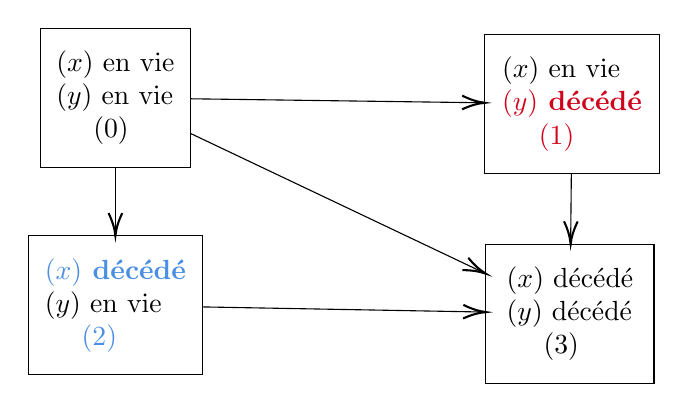
\begin{tikzpicture}[x=0.75pt,y=0.75pt,yscale=-1,xscale=1]
%uncomment if require: \path (0,300); %set diagram left start at 0, and has height of 300


% Text Node
\draw    (177,28.5) -- (249,28.5) -- (249,95.5) -- (177,95.5) -- cycle  ;
\draw (213,62) node  [align=left] {$\displaystyle ( x)$ en vie\\$\displaystyle ( y)$ en vie \\ \ \ \ \ $\displaystyle ( 0)$};
% Text Node
\draw    (391,31.5) -- (475,31.5) -- (475,98.5) -- (391,98.5) -- cycle  ;
\draw (433,65) node  [align=left] {$\displaystyle ( x)$ en vie \\\textcolor[rgb]{0.82,0.01,0.11}{$\displaystyle ( y)$\textbf{ décédé}} \\ \ \ \ \ \textcolor[rgb]{0.82,0.01,0.11}{$\displaystyle ( 1)$}};
% Text Node
\draw    (171,128.5) -- (255,128.5) -- (255,195.5) -- (171,195.5) -- cycle  ;
\draw (213,162) node  [align=left] {\textcolor[rgb]{0.29,0.56,0.89}{$\displaystyle ( x)$\textbf{ décédé}} \\$\displaystyle ( y)$ en vie \\ \ \ \ \ \textcolor[rgb]{0.29,0.56,0.89}{$\displaystyle ( 2)$}};
% Text Node
\draw    (391.5,132.5) -- (472.5,132.5) -- (472.5,199.5) -- (391.5,199.5) -- cycle  ;
\draw (432,166) node  [align=left] {$\displaystyle ( x)$ décédé \\$\displaystyle ( y)$ décédé \\ \ \ \ \ $\displaystyle ( 3)$};
% Connection
\draw    (249,62.49) -- (389,64.4) ;
\draw [shift={(391,64.43)}, rotate = 180.78] [color={rgb, 255:red, 0; green, 0; blue, 0 }  ][line width=0.75]    (10.93,-3.29) .. controls (6.95,-1.4) and (3.31,-0.3) .. (0,0) .. controls (3.31,0.3) and (6.95,1.4) .. (10.93,3.29)   ;

% Connection
\draw    (432.67,98.5) -- (432.35,130.5) ;
\draw [shift={(432.33,132.5)}, rotate = 270.57] [color={rgb, 255:red, 0; green, 0; blue, 0 }  ][line width=0.75]    (10.93,-3.29) .. controls (6.95,-1.4) and (3.31,-0.3) .. (0,0) .. controls (3.31,0.3) and (6.95,1.4) .. (10.93,3.29)   ;

% Connection
\draw    (249,79.1) -- (389.69,145.91) ;
\draw [shift={(391.5,146.77)}, rotate = 205.4] [color={rgb, 255:red, 0; green, 0; blue, 0 }  ][line width=0.75]    (10.93,-3.29) .. controls (6.95,-1.4) and (3.31,-0.3) .. (0,0) .. controls (3.31,0.3) and (6.95,1.4) .. (10.93,3.29)   ;

% Connection
\draw    (213,95.5) -- (213,126.5) ;
\draw [shift={(213,128.5)}, rotate = 270] [color={rgb, 255:red, 0; green, 0; blue, 0 }  ][line width=0.75]    (10.93,-3.29) .. controls (6.95,-1.4) and (3.31,-0.3) .. (0,0) .. controls (3.31,0.3) and (6.95,1.4) .. (10.93,3.29)   ;

% Connection
\draw    (255,162.77) -- (389.5,165.22) ;
\draw [shift={(391.5,165.26)}, rotate = 181.05] [color={rgb, 255:red, 0; green, 0; blue, 0 }  ][line width=0.75]    (10.93,-3.29) .. controls (6.95,-1.4) and (3.31,-0.3) .. (0,0) .. controls (3.31,0.3) and (6.95,1.4) .. (10.93,3.29)   ;


\end{tikzpicture}









% -------------------------------------------------------------
% Fin de la feuille aide-mémoire
\end{multicols*}
\end{document}
